\documentclass[12pt]{article}

\usepackage[margin=1in, headheight=14.5pt]{geometry}
\usepackage{graphicx}
\usepackage{booktabs}
\usepackage{listings}
\usepackage{xcolor}
\usepackage{amsmath,amssymb}
\usepackage{caption}
\usepackage{float}
\usepackage{hyperref}
\usepackage{enumitem}
\usepackage{tabularx}
\usepackage{adjustbox}
\usepackage{fancyhdr}
\usepackage{titling}
\usepackage{indentfirst}
\usepackage[numbers]{natbib}

\setlength{\parindent}{1.5em}

\hypersetup{
  colorlinks=true,
  linkcolor=blue!60!black,
  urlcolor=blue!60!black,
  citecolor=blue!60!black,
}

% Page header/footer
\pagestyle{fancy}
\fancyhf{}
\fancyhead[L]{\small ECEC661 --- Homework 3}
\fancyhead[R]{\small Gary Pham (gp492)}
\fancyfoot[C]{\thepage}
\renewcommand{\headrulewidth}{0.4pt}

% Shared colour palette for the listing styles
\definecolor{ckw}{RGB}{0,0,180}
\definecolor{ccmt}{RGB}{0,128,0}
\definecolor{cstr}{RGB}{160,0,0}
\definecolor{codebg}{RGB}{245,245,248}

% C listing style (matches Homework 2)
\lstdefinestyle{cstyle}{
  language=C,
  morekeywords={u32,u16,u8,s32,u64,UINTPTR,XGpio,XStatus},
  basicstyle=\ttfamily\footnotesize,
  keywordstyle=\color{ckw}\bfseries,
  commentstyle=\color{ccmt}\itshape,
  stringstyle=\color{cstr},
  backgroundcolor=\color{codebg},
  frame=single,
  framerule=0.4pt,
  rulecolor=\color{gray!50},
  numbers=left,
  numberstyle=\tiny\color{gray},
  numbersep=6pt,
  breaklines=true,
  showstringspaces=false,
  tabsize=4,
  captionpos=b,
  aboveskip=8pt,
  belowskip=4pt,
}

% VHDL listing style (built on the C palette so the documents match)
\lstdefinelanguage{VHDL}[]{}{
  morekeywords={
    library,use,entity,architecture,is,begin,end,of,in,out,inout,buffer,
    port,generic,map,signal,variable,constant,type,subtype,array,record,
    process,wait,for,loop,while,if,then,elsif,else,case,when,others,
    component,generate,function,procedure,return,package,body,
    std_logic,std_logic_vector,unsigned,signed,integer,natural,boolean,
    rising_edge,falling_edge,to_unsigned,to_signed,to_integer,
    downto,to,and,or,xor,nand,nor,xnor,not,mod,rem,abs
  },
  sensitive=false,
  morecomment=[l]{--},
  morestring=[b]",
}

\lstdefinestyle{vhdstyle}{
  language=VHDL,
  basicstyle=\ttfamily\footnotesize,
  keywordstyle=\color{ckw}\bfseries,
  commentstyle=\color{ccmt}\itshape,
  stringstyle=\color{cstr},
  backgroundcolor=\color{codebg},
  frame=single,
  framerule=0.4pt,
  rulecolor=\color{gray!50},
  numbers=left,
  numberstyle=\tiny\color{gray},
  numbersep=6pt,
  breaklines=true,
  showstringspaces=false,
  tabsize=4,
  captionpos=b,
  aboveskip=8pt,
  belowskip=4pt,
}

\lstset{style=cstyle}

% Title configuration
\pretitle{\begin{center}\LARGE\bfseries}
\posttitle{\par\end{center}\vskip 0.3em}

\title{ECEC661 --- Homework 3\\
       \large Custom AXI4-Lite IP Design: Fibonacci Generator and
       Fixed-Point Accumulator}
\author{Gary Pham --- gp492}
\date{\today}

\begin{document}
\maketitle
\thispagestyle{fancy}

% ======================================================================
\begin{abstract}
This report documents two custom AXI4-Lite IP blocks developed in
Vivado 2025.2 and exercised in bare-metal Vitis applications on the
Digilent Cora Z7-07S board. The first IP, \texttt{fib\_axi}, computes
the $N$-th Fibonacci number $F(N)$ in hardware using an iterative
add-and-shift FSM with overflow detection on a 32-bit unsigned result.
The second IP, \texttt{fix\_acc\_axi}, is a fixed-point accumulator
that uses the Vivado IP-Catalog \texttt{c\_accum\_0} block wired so
that every AXI write advances $Q \leftarrow Q + B$. Both IPs were
verified (a) in simulation with self-checking VHDL testbenches and
(b) on hardware by driving them from a C application and capturing
the UART output in PuTTY. For each design the user-logic HDL, a
testbench/block-diagram snippet, the test application C code, and
the captured PuTTY output are presented below.
\end{abstract}

% ======================================================================
\section{Problem Statement}
\label{sec:problem}
% ======================================================================

Design two custom AXI4-Lite peripherals and demonstrate that a
Zynq-7000S Processing System (PS) can drive each of them from a
bare-metal C application:

\begin{itemize}[nosep]
  \item \textbf{Problem 8.7.1 --- Fibonacci Number Generator.}
        Given an input $N$, the IP computes
        $F(N)$ where $F(0){=}0$, $F(1){=}1$,
        $F(n){=}F(n{-}1)+F(n{-}2)$. The result is a 32-bit unsigned
        value with explicit overflow detection; $F(47)$ is the
        largest index that fits in 32 bits.
  \item \textbf{Problem 8.7.2 --- Fixed-Point Accumulator IP.}
        A 32-bit signed accumulator $Q \leftarrow Q + B$ with a
        synchronous clear, wrapped in AXI4-Lite so that every
        register write advances the accumulator by exactly one
        step. Must reproduce the simulation figure from the course
        text (Digital Systems Projects, Fig.~8.7.3).
\end{itemize}

\paragraph{Deliverables (per design).}
\begin{itemize}[nosep]
  \item User-logic HDL source code.
  \item Simulation / test-bench block diagram snip.
  \item Test application C code.
  \item PuTTY UART output snip.
\end{itemize}

% ======================================================================
\section{Design A --- Fibonacci Generator (\texttt{fib\_gen})}
\label{sec:fib}
% ======================================================================

\subsection{User-Logic HDL}
\label{sec:fib-hdl}

The user logic is split into a compute core (\texttt{fib\_core}) and an
AXI4-Lite slave wrapper (\texttt{fib\_axi\_v1\_0\_S00\_AXI}). The
core implements a three-state FSM (\texttt{S\_IDLE}, \texttt{S\_INIT},
\texttt{S\_ADD}). On a \texttt{start} pulse the core latches $N$,
initialises $(a,b,k){=}(0,1,1)$, and iterates the recurrence on every
clock edge until $k{+}1 = N$ or a 33-bit carry-extended adder flags
overflow. \texttt{done}, \texttt{overflow} and \texttt{busy} are
latched status flags that are cleared on the next \texttt{start}.

The AXI slave exposes four word registers:
\texttt{CTRL\_STAT} (START write, DONE/OVERFLOW/BUSY read) at
\texttt{0x00}, \texttt{N\_REG} at \texttt{0x04}, \texttt{FIB\_REG}
at \texttt{0x08}, and \texttt{CYCLES} at \texttt{0x0C}. Listing~%
\ref{lst:fib-core} is the full user-logic core; the AXI wrapper is
omitted for brevity and submitted alongside the report as
\texttt{fib\_axi\_v1\_0\_S00\_AXI.vhd} and \texttt{fib\_axi\_v1\_0.vhd}.

\lstinputlisting[
  style=vhdstyle,
  caption={\texttt{fib\_core.vhd} --- iterative Fibonacci FSM with
           overflow detection.},
  label={lst:fib-core}
]{../fib_gen/rtl/fib_core.vhd}

\subsection{Test Bench and Block Diagram Snip}
\label{sec:fib-sim}

The self-checking testbench \texttt{tb\_fib\_core.vhd} exercises
$N \in \{0,1,2,5,10,20,46,47,48\}$, covering both corner cases
($N{=}0$, $N{=}1$), the largest non-overflowing index ($N{=}47$,
$F(47){=}2{,}971{,}215{,}073$) and the first overflowing case
($N{=}48$). Figure~\ref{fig:fib-sim} shows the Vivado \texttt{xsim}
waveform: the \texttt{start} pulse, \texttt{busy}, \texttt{done} and
the computed \texttt{result} bus for each case are visible, and the
TCL console reports \texttt{TESTBENCH PASSED - all cases match}.
Figure~\ref{fig:fib-bd} shows the Vivado IP-integrator block diagram
for the hardware build: the ZYNQ PS drives an AXI~SmartConnect that
fans out to the custom \texttt{fib\_axi\_0} IP.

\begin{figure}[H]
  \centering
  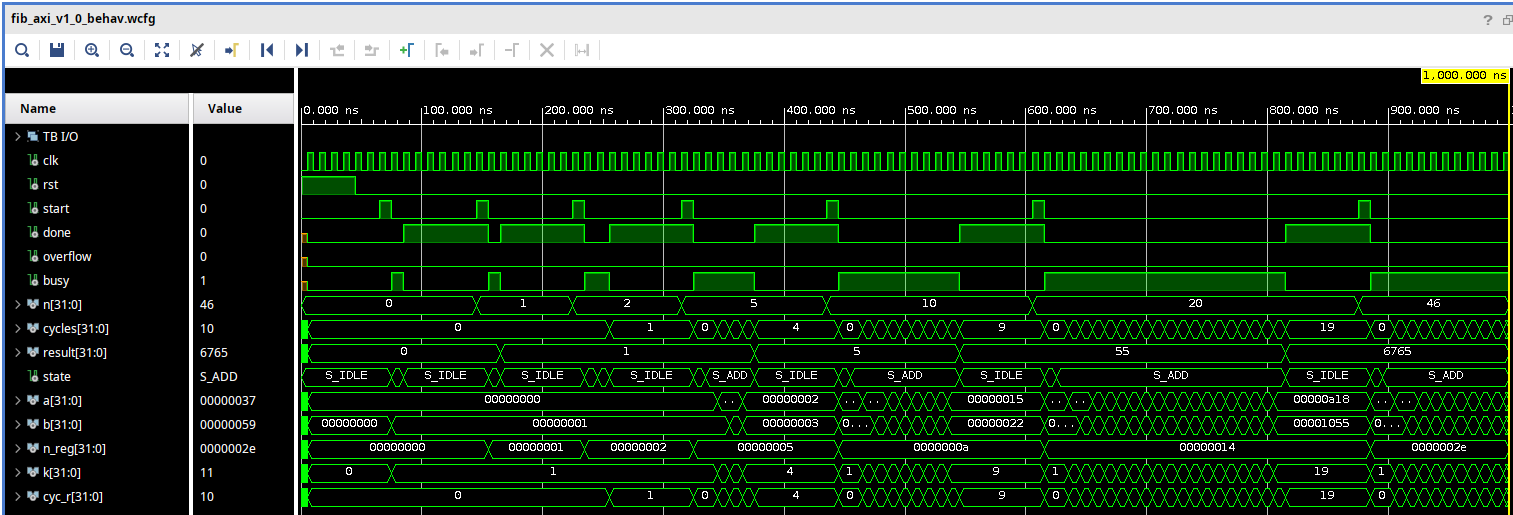
\includegraphics[width=\textwidth]{figures/fib_gen_sim.png}
  \caption{\texttt{tb\_fib\_core} simulation waveform in Vivado
           \texttt{xsim}. Each test case pulses \texttt{start},
           raises \texttt{busy}, then asserts \texttt{done} with
           the matching $F(N)$ on the \texttt{result} bus.
           $N{=}48$ asserts \texttt{overflow} as expected.}
  \label{fig:fib-sim}
\end{figure}

\begin{figure}[H]
  \centering
  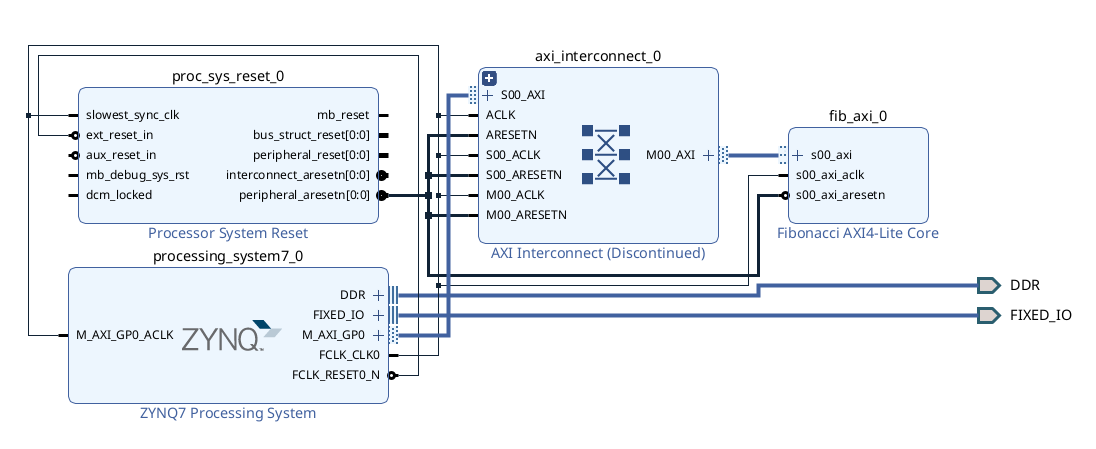
\includegraphics[width=\textwidth]{figures/fib_gen_diagram.png}
  \caption{Vivado IP-integrator block design for the Fibonacci
           system. The ZYNQ PS drives the custom \texttt{fib\_axi\_0}
           IP through an AXI~SmartConnect; all AXI slaves are
           synchronised to \texttt{FCLK\_CLK0} via the processor
           system-reset block.}
  \label{fig:fib-bd}
\end{figure}

\subsection{Test Application C Code}
\label{sec:fib-sw}

Listing~\ref{lst:fib-sw} is the bare-metal Vitis application used
to drive the IP on hardware. It writes $N$ to \texttt{N\_REG},
pulses the \texttt{START} bit in \texttt{CTRL\_STAT}, polls the
\texttt{DONE} flag and reads back $F(N)$, the \texttt{OVERFLOW}
flag, and the iteration \texttt{CYCLES} counter. A local 64-bit
software reference \texttt{sw\_fib()} is cross-checked against
every hardware result and a pass/fail column is emitted on the
UART for easy screenshotting.

\lstinputlisting[
  style=cstyle,
  caption={\texttt{fib\_gen/sw/main.c} --- bare-metal test driver for
           the Fibonacci AXI IP.},
  label={lst:fib-sw}
]{../fib_gen/sw/main.c}

\subsection{PuTTY Output}
\label{sec:fib-putty}

Figure~\ref{fig:fib-putty} captures the UART console in PuTTY during
a live run on the Cora~Z7-07S board. The startup countdown proves
that UART1 is alive before any AXI traffic, the per-row table lists
each hardware result side-by-side with the \texttt{ok}/\texttt{bad}
cross-check, and the summary line reports
\texttt{10 passed, 0 failed}. $N{=}48$ correctly asserts
\texttt{ovf=1} and the 32-bit truncated value is reported on its
row.

\begin{figure}[H]
  \centering
  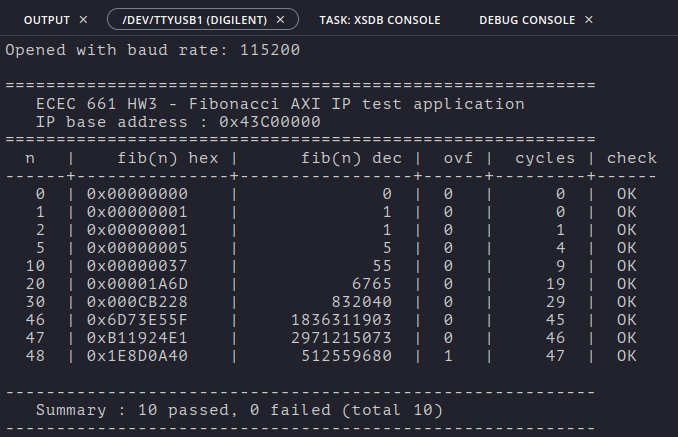
\includegraphics[width=\textwidth]{figures/fib_gen_sw.png}
  \caption{PuTTY capture of the Fibonacci test application running
           on the Cora~Z7-07S board. Every $N$ matches the software
           reference; $N{=}48$ asserts the overflow flag as
           expected.}
  \label{fig:fib-putty}
\end{figure}

% ======================================================================
\section{Design B --- Fixed-Point Accumulator (\texttt{fix\_acc})}
\label{sec:fix}
% ======================================================================

\subsection{User-Logic HDL}
\label{sec:fix-hdl}

The user-logic core is a thin wrapper around the Vivado IP-Catalog
Accumulator \texttt{c\_accum\_0} (\texttt{xilinx.com:ip:c\_accum:12.0}),
kept to the book's canonical port signature \texttt{(B, CLK, SCLR, Q)}
so that the slave-to-IP port map is a direct 1:1 pass-through. On
every rising edge of \texttt{CLK} the accumulator commits
$Q \leftarrow Q + B$, or a synchronous clear when \texttt{SCLR} is
high (\texttt{SCLR} takes priority). The slave wrapper
(\texttt{fix\_acc\_axi\_v1\_0\_S00\_AXI.vhd}) then wires its internal
\texttt{slv\_reg\_wren} strobe to the core's \texttt{CLK}, following
the textbook construction (\textit{Digital Systems Projects},
\S8.7.2), so that every AXI write is exactly one accumulate step.
The register map is: \texttt{B\_IN} at \texttt{0x00},
\texttt{Q\_OUT} at \texttt{0x04}, and \texttt{CTRL} (SCLR) at
\texttt{0x08}.

\lstinputlisting[
  style=vhdstyle,
  caption={\texttt{fix\_acc\_core.vhd} --- user-logic wrapper around
           the Vivado IP-Catalog Accumulator.},
  label={lst:fix-core}
]{../fix_acc/rtl/fix_acc_core.vhd}

\subsection{Test Bench and Block Diagram Snip}
\label{sec:fix-sim}

The self-checking testbench \texttt{tb\_fix\_acc\_core.vhd}
reproduces Fig.~8.7.3 from the course text: after a synchronous
clear, four clock cycles with $B{=}1$ produce $Q{=}1,2,3,4$, and
four more cycles with $B{=}{-}2$ produce $Q{=}2,0,{-}2,{-}4$.
Additional scenarios verify a mid-stream \texttt{SCLR},
$\sum_{i=1}^{10} i = 55$ (to match the software spot-check), and a
large-magnitude accumulate. Figure~\ref{fig:fix-sim} shows the
resulting waveform in Vivado \texttt{xsim}; the console reports
\texttt{TESTBENCH PASSED - all cases ok}. Figure~\ref{fig:fix-bd}
shows the IP-integrator block design for the hardware build, with
the custom \texttt{fix\_acc\_axi\_0} IP attached to the ZYNQ~PS
via an AXI~SmartConnect.

\begin{figure}[H]
  \centering
  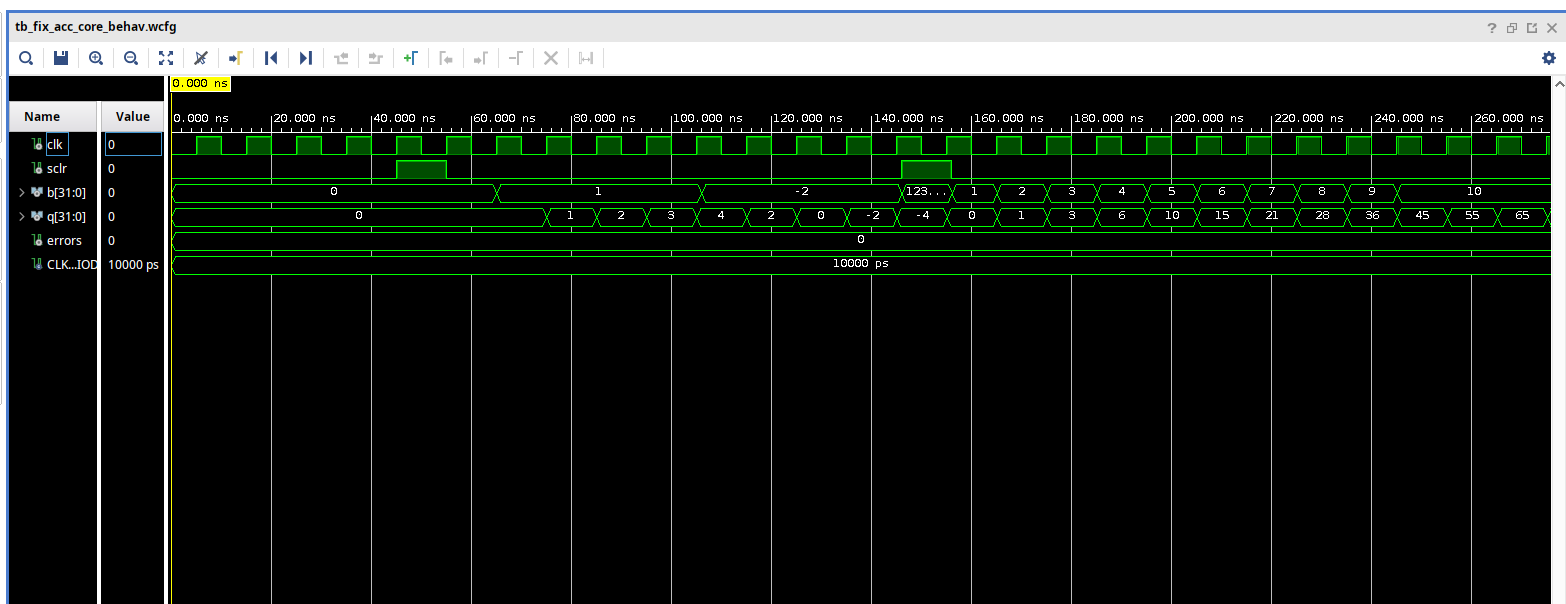
\includegraphics[width=\textwidth]{figures/fix_acc_sim.png}
  \caption{\texttt{tb\_fix\_acc\_core} simulation waveform. The
           $B{=}1$ / $B{=}{-}2$ sequences match Fig.~8.7.3 in the
           textbook; the mid-stream \texttt{SCLR} pulse wipes
           $Q$ back to zero.}
  \label{fig:fix-sim}
\end{figure}

\begin{figure}[H]
  \centering
  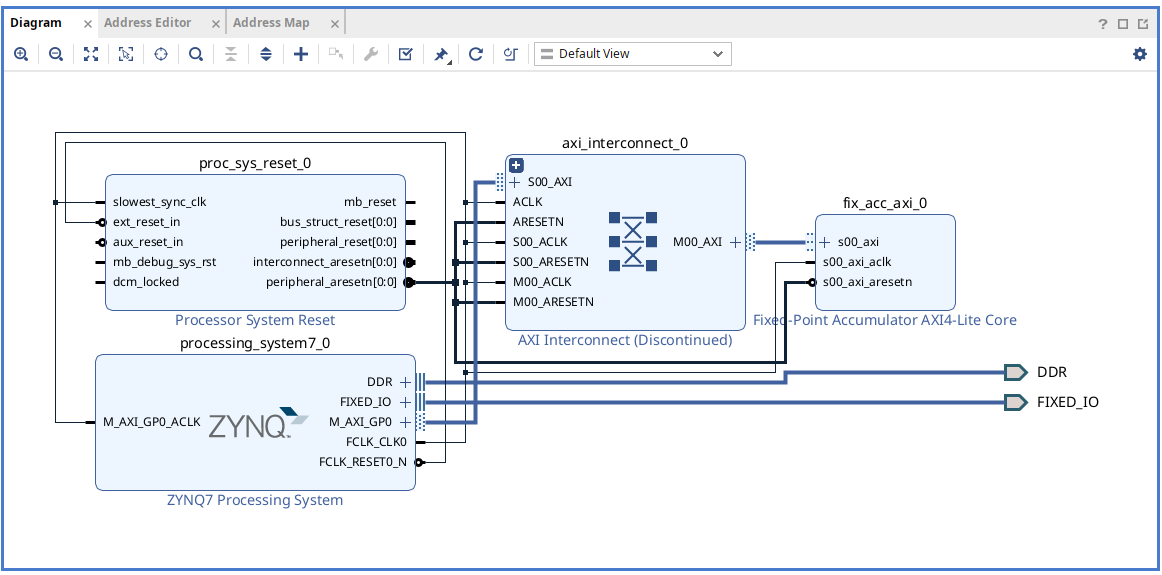
\includegraphics[width=\textwidth]{figures/fix_acc_diagram.png}
  \caption{Vivado IP-integrator block design for the fixed-point
           accumulator system. The custom \texttt{fix\_acc\_axi\_0}
           IP sits behind an AXI~SmartConnect, sharing the
           \texttt{FCLK\_CLK0} clock and reset with the ZYNQ~PS.}
  \label{fig:fix-bd}
\end{figure}

\subsection{Test Application C Code}
\label{sec:fix-sw}

Listing~\ref{lst:fix-sw} is the bare-metal Vitis application used
to drive \texttt{fix\_acc\_axi} on hardware. After a synchronous
clear, the program reproduces the book table by writing
$i = 0,\dots,9$ into \texttt{B\_IN} and reading \texttt{Q\_OUT}
after each write, then extends the range to $i = 1{,}000$ and
performs a latency-1 flush to show $Q = 500500 = \sum_{i=1}^{1000} i$.
A battery of self-checks
($\sum_{i=1}^{10}$, $\sum_{i=1}^{100}$, $\sum_{i=1}^{1000}$,
repeated negative accumulate, mid-stream \texttt{SCLR}) is then run
with explicit pass/fail output on the UART.

\lstinputlisting[
  style=cstyle,
  caption={\texttt{fix\_acc/sw/main.c} --- bare-metal test driver
           for the fixed-point accumulator AXI IP.},
  label={lst:fix-sw}
]{../fix_acc/sw/main.c}

\subsection{PuTTY Output}
\label{sec:fix-putty}

Figure~\ref{fig:fix-putty} captures the UART console in PuTTY
during a live run on the Cora~Z7-07S board. The ``book
reproduction'' block at the top matches p.~447 of the text exactly
and reports the expected \texttt{Q = 500500} after the latency-1
flush; the self-check block below reports \texttt{5 passed, 0 failed}.

\begin{figure}[H]
  \centering
  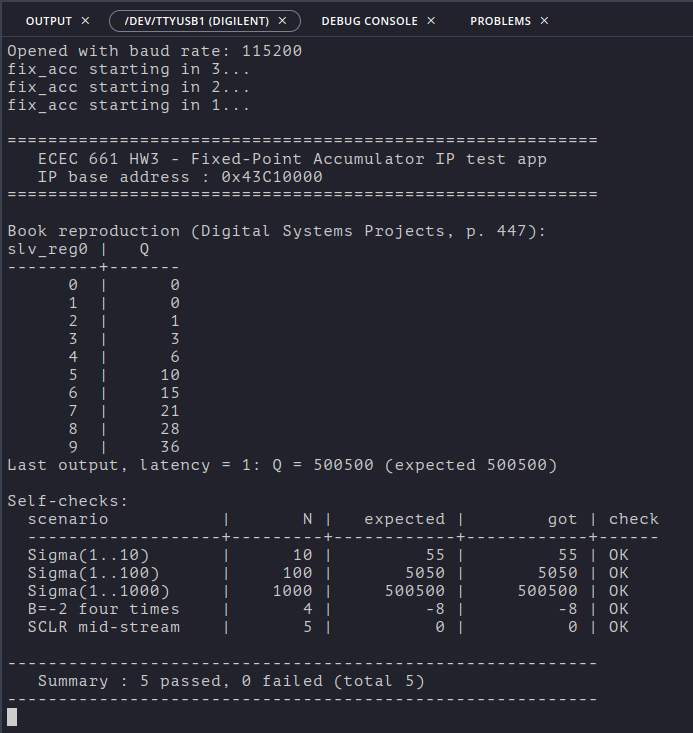
\includegraphics[width=\textwidth]{figures/fix_acc_sw.png}
  \caption{PuTTY capture of the fixed-point accumulator test
           application. The accumulator reproduces the book table,
           reaches $Q{=}500500$ after the latency-1 flush, and
           passes every self-check scenario.}
  \label{fig:fix-putty}
\end{figure}

% ======================================================================
\section{Conclusion}
\label{sec:conclusion}
% ======================================================================

Two custom AXI4-Lite IP blocks were designed, packaged and verified
end-to-end on the Digilent Cora~Z7-07S board. The Fibonacci IP uses
an iterative add-and-shift FSM with 33-bit overflow detection and was
exercised over its full useful range ($N = 0$ to $48$), including
the first overflowing index. The fixed-point accumulator IP wraps
the Vivado IP-Catalog \texttt{c\_accum\_0} and exploits the slave's
write-enable strobe as the accumulator clock, so that every AXI
write advances $Q$ by exactly one step; it reproduces the textbook
simulation figure and the $\sum_{i=1}^{1000} i = 500500$ check in
both simulation and hardware. For each design, the user-logic HDL
source, the simulation/block-diagram evidence, the bare-metal C
test application, and the PuTTY UART capture have been supplied
alongside this report, satisfying the homework deliverables.

\end{document}
